\section{How is EdgeRock built?}
\label{sec:architecture}

\subsection{Decoder layout}

EdgeRock-4B adapts the Qwen3.5-4B language backbone~\cite{qwen35}. It retains 24 Gated DeltaNet (GDN) layers and replaces its eight full-attention layers with a 1,024-position sliding window~\cite{longformer} plus an independent Rock Memory Anchors (RMA) module. The resulting pattern is
\begin{equation}
\bigl[\mathrm{GDN},\ \mathrm{GDN},\ \mathrm{GDN},\ \mathrm{SWA}_{1024}\parallel\mathrm{RMA}\bigr]\times8.
\end{equation}
Every sequence mixer is followed by a feed-forward sublayer; each of the eight RMA modules has its own parameters and state. Image features from the visual encoder and merger join text embeddings in a shared decoder input sequence (Figure~\ref{fig:architecture}a).

\begin{figure}[!tbp]
\centering
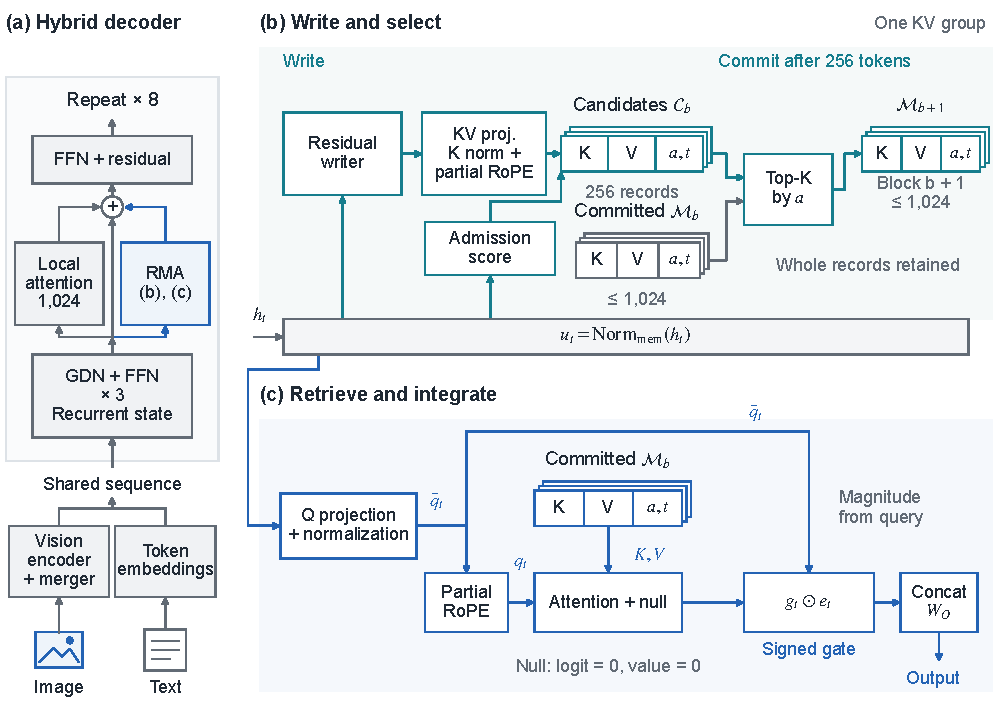
\includegraphics[width=\linewidth]{architecture_overview.pdf}
\caption{\textbf{EdgeRock architecture.} \textbf{(a)} Text and image features share a decoder combining recurrence, local attention, and Rock Memory Anchors (RMA). \textbf{(b)} Per KV group, admission selects up to 1,024 records from the committed bank and 256 writer-generated candidates. Selections become readable in the next block. \textbf{(c)} Current queries read committed anchors; null attention and a query-conditioned signed gate control their contribution to the residual stream alongside local attention.}
\label{fig:architecture}
\end{figure}

GDN uses fixed-dimensional recurrent matrices~\cite{gateddeltanet}. The local window and anchor bank retain separate KV records; a source position may appear in both.

\Needspace{12\baselineskip}
\subsection{Fixed capacity, adaptive content}

EdgeRock keeps the size of its persistent history constant and updates only its contents. Let $t=0,1,\ldots$ index causal sequence positions and $b(t)=\lfloor t/C\rfloor$ identify the current candidate block of $C=256$ positions. Immediately before position $t$,
\begin{align}
\mathcal H_t&=(\mathcal R_t,\mathcal L_t,\mathcal M_{b(t)},\mathcal C_t,\pi_t),\label{eq:history-state}\\
(y_t,\mathcal H_{t+1})&=F_\theta(x_t,\mathbf p_t,\mathcal H_t).\label{eq:history-transition}
\end{align}
Here $x_t$ is the input embedding, $y_t$ is the decoder output, and $\mathbf p_t$ contains the rotary coordinates. Across the decoder, $\mathcal R_t$ collects recurrent states, $\mathcal L_t$ local KV, $\mathcal M_{b(t)}$ committed anchor banks, $\mathcal C_t$ pending candidates, and $\pi_t$ progress metadata.

\subsection{Integration into the reasoning computation}

Suppressing layer indices, each local-plus-RMA layer integrates retrieved information into the residual stream alongside local attention:
\begin{align}
z_t &= h_t+\mathrm{SWA}(\mathrm{Norm}_{\mathrm{local}}(h_t))+\mathrm{RMA}(h_t,\mathcal M_{b(t)}),\\
h_t^{\mathrm{out}} &= z_t+\mathrm{MLP}(\mathrm{Norm}_{\mathrm{ffn}}(z_t)).
\end{align}
RMA uses independent normalization, writing, admission, query, key, and value projections, and output projection. The residual $z_t$ carries local and retrieved information to later layers.

\begin{table}[!htbp]
\centering\small
\caption{EdgeRock-4B configuration.}
\label{tab:architecture}
\begin{tabularx}{\linewidth}{@{}YlYl@{}}
\toprule
Quantity & Value & Quantity & Value\\
\midrule
Model scale & 4B & RMA parameters & 372M\\
Recurrent / local-plus-RMA layers & 24 / 8 & Residual width & 2,560\\
Attention query heads / KV groups & 16 / 4 & Attention head dimension & 256\\
Local window $W$ & 1,024 & Committed capacity $K$ & 1,024\\
Candidate block $C$ & 256 & RMA KV precision & BF16\\
\bottomrule
\end{tabularx}
\end{table}

\FloatBarrier
\subsection{Staged conversion}
\label{sec:training}
EdgeRock-4B is converted from Qwen3.5-4B in four stages. RMA adaptation (M0) teaches the new RMA modules to retain and retrieve information needed for later predictions. Joint adaptation (R) trains RMA together with the recurrent and local-attention backbone, so downstream layers learn to use what is retrieved. Supervised post-training (S) develops general-purpose responses with the adapted history mechanism, and reinforcement learning with verifiable rewards (RLVR)~\cite{tulu3,deepseekr1} refines responses using feedback on answer correctness and task completion. Section~\ref{sec:diagnostic} tracks memory accuracy after each stage (Figure~\ref{fig:memory}a).

\section{How do Rock Memory Anchors preserve distant information?}
\label{sec:memory-algorithm}

At each token, RMA reads the committed anchor bank and produces a candidate record from the same causal input. At each block boundary, admission selects records from the bank and the new candidates; the updated bank becomes readable in the next block. Local attention covers recent tokens while candidates accumulate. Algorithm~\ref{alg:anchor-update} in Appendix~\ref{sec:streaming-execution} gives the complete per-token procedure.

\subsection{Independent memory writer}
\label{sec:write}

Let $u_t=\mathrm{Norm}_{\mathrm{mem}}(h_t)\in\mathbb R^D$, with $D=2{,}560$. An independent residual writer with a SwiGLU-style gated projection~\cite{glu} constructs a storage representation:
\begin{equation}
w_t = u_t+W_{\mathrm{down}}\!\left[\mathrm{SiLU}(W_{\mathrm{gate}}u_t)\odot W_{\mathrm{up}}u_t\right].
\end{equation}
RMA KV projections use the writer output $w_t$; query projections use $u_t$. The writer has an intermediate width of 2,560~\cite{edgerockcode,edgerockconfig}.

\subsection{Causal admission in four independent KV groups}

A small network assigns a retention priority to each KV group:
\begin{equation}
a_t = W_{a,2}\,\mathrm{SiLU}(W_{a,1}u_t),\qquad a_t\in\mathbb R^4.
\end{equation}
Bias-free projections of size $2560\!\rightarrow\!256\!\rightarrow\!4$ compute FP32 scores from the current causal context~\cite{edgerockcode,edgerockconfig}. Each group independently retains its highest-scoring records; source positions may overlap across groups.

\subsection{Blockwise commits and causal visibility}

Every 256 tokens, the committed bank and new candidates compete for 1,024 slots per KV group.

For block $\mathcal B_b=\{bC,\ldots,(b+1)C-1\}$, group $g$, capacity $K=1024$ and block size $C=256$,
\begin{align}
\mathcal C_{b,g}&=\{(k_{t,g},v_{t,g},a_{t,g},t):t\in\mathcal B_b\},\\
\mathcal M_{b+1,g}&=\operatorname{TopK}_{a_g}(\mathcal M_{b,g}\cup\mathcal C_{b,g};K).
\end{align}
During block $b$, queries read $\mathcal M_{b,g}$; selected candidates become readable in block $b+1$. The 1,024-position local window covers current-block interactions while the 256-token candidate buffer fills. Each update inspects at most $K+C=1280$ records per group and then reuses the candidate buffer.

The operator $\operatorname{TopK}(A;K)$ retains up to $K$ records, ordered by descending score and then earlier causal position. With fixed write-time scores, the committed bank satisfies the exact history invariant
\begin{equation}
\mathcal M_{b,g}=\operatorname{TopK}_{a_g}\!\left(\bigcup_{r=0}^{b-1}\mathcal C_{r,g};K\right),
\qquad \mathcal M_{0,g}=\varnothing.
\label{eq:history-topk}
\end{equation}
Every discarded record already has at least $K$ records ahead of it, so later candidates cannot bring it into the global top $K$. The update therefore maintains the highest-priority records from all completed blocks using bounded storage. Capacity limits record count, not retention age: a record remains directly addressable until displaced by admission.

\Needspace{10\baselineskip}
\subsection{Query-dependent retrieval from the anchor bank}
\label{sec:read}

A later query can address any retained record, including one whose source position has left the local window. Each module uses 16 query heads over four KV groups~\cite{gqa}, with head dimension $d=256$. Queries and keys use learned RMS normalization~\cite{rmsnorm,edgerockcode,edgerockconfig}:
\begin{equation}
\operatorname{RMS}_{\gamma}(x)=\frac{\gamma\odot x}{\sqrt{d^{-1}\sum_{i=1}^{d}x_i^2+10^{-6}}}.
\end{equation}
The query reads the current representation $u_t$; keys and values store the writer representation $w_t$:
\begin{align}
\bar q_{t,h}&=\operatorname{RMS}_{\gamma_Q}(W_{Q,h}u_t),
&q_{t,h}&=R(\mathbf p_t)\bar q_{t,h},\\
k_{t,g}&=R(\mathbf p_t)\operatorname{RMS}_{\gamma_K}(W_{K,g}w_t),
&v_{t,g}&=W_{V,g}w_t.
\label{eq:memory-qkv}
\end{align}
Each projection $W_{Q,h},W_{K,g},W_{V,g}\in\mathbb R^{d\times D}$. Query and key gains are separate and shared across heads or groups within a module, with effective gain $\gamma=1+\omega$. The partial rotary transform~\cite{roformer} $R(\mathbf p_t)$ rotates 64 of 256 coordinates with base $10^7$; values are stored without this transform or Q/K normalization. Text-only input uses $\mathbf p_t=(t,t,t)$, while multimodal input uses the backbone's spatial and temporal coordinates (Appendix~\ref{sec:streaming-execution}).

For head $h$, assigned to KV group $g(h)$, let $\mathcal I_{b,g}$ index the records in $\mathcal M_{b,g}$ and define $\ell_{tj,h}=q_{t,h}^{\top}k_{j,g(h)}/\sqrt d$. With $b=b(t)$, the committed-bank read is
\begin{equation}
e_{t,h}=\sum_{j\in\mathcal I_{b,g(h)}}
\frac{\exp(\ell_{tj,h})}
{1+\sum_{i\in\mathcal I_{b,g(h)}}\exp(\ell_{ti,h})}\,v_{j,g(h)}.
\end{equation}
Each head reads at most 1,024 records. Query heads share each group's KV bank but compute distinct attention weights.

\paragraph{Retrieval content and strength.}
The null item has zero logit and value. Its attention mass is $\alpha_{0,t,h}=(1+Z_{t,h})^{-1}$, with $Z_{t,h}=\sum_{j\in\mathcal I_{b,g(h)}}\exp(\ell_{tj,h})$. For a nonempty bank, the read factors into
\begin{equation}
e_{t,h}=(1-\alpha_{0,t,h})\,\bar v_{t,h},
\qquad
\bar v_{t,h}=\sum_{j\in\mathcal I_{b,g(h)}}
\frac{\exp(\ell_{tj,h})}{Z_{t,h}}\,v_{j,g(h)}.
\label{eq:retrieval-factorization}
\end{equation}
The query determines both the retrieved content $\bar v_{t,h}$ and the total mass assigned to memory. The read lies in the convex hull of the stored values and zero; an empty bank returns exactly zero.

\subsection{Query-conditioned memory output}
The output gate acts on each retrieved head:
\begin{align}
g_{t,h}&=\tanh(s_h)\,2\sigma\!\left(\frac{\bar q_{t,h}^{\top}b_h}{\sqrt d}+c_h\right),\\
\mathrm{RMA}(h_t,\mathcal M_{b(t)})&=W_O\,\operatorname{concat}_{h}\!\left(g_{t,h}e_{t,h}\right).
\end{align}
Here $\bar q$ is the normalized query before rotary encoding; $s_h,c_h\in\mathbb R$, $b_h\in\mathbb R^d$, and $W_O\in\mathbb R^{D\times16d}$ are learned parameters. The gate is a signed multiplier in $(-2,2)$. Its sign comes from the learned scale $\tanh(s_h)$; the query-conditioned sigmoid modulates its magnitude.

Admission determines which records are available, retrieval determines their content and attention mass, and the signed gate controls their contribution to the residual stream.

\paragraph{Relation to other retained-memory designs.}
Several designs also keep a small set of key--value records next to a compressed or local history. AnLLM trains a model to summarize each text segment into an anchor token and keep only those tokens' keys and values~\cite{anllm}; its anchors still accumulate as the sequence grows. HOLA adds to a linear-attention model a bounded cache of recurrent keys and values ranked by a fixed, parameter-free priority~\cite{hola}, and LTE learns per-head scores that decide which tokens to retain as they leave a sliding window~\cite{lte}. RMA differs in three ways: an independent writer produces dedicated records rather than copying existing keys and values; a causal scorer admits them into a fixed-size bank through per-group top-$K$ commits every 256 tokens; and a separately normalized, gated read integrates them alongside local attention in a converted reasoning model.

\section{What stays constant as context grows?}
\label{sec:complexity}

Fixed-size recurrent state, the local window, and anchor banks bound both stored history and per-token history access.

\subsection{Memory that does not grow with sequence length}

For prompt length $P$ and generated length $N$, hold model dimensions, layer counts, precision, local window $W$, memory capacity $K$ and block size $C$ fixed. Storage counts fixed-width tensor elements and metadata words. The complete persistent history allocation is
\begin{equation}
S_{\mathrm{history}}=S_{\mathrm{GDN}}+S_{\mathrm{SWA}}+S_{\mathrm{committed}}+S_{\mathrm{candidates}}+S_{\mathrm{metadata}}.
\end{equation}
Recurrent matrices, the local ring, committed anchor banks, pending candidates, scores and indices all have bounded capacity. The history allocation is consequently $O(1)$ in $P+N$ for each sequence.

\begin{align}
S_{\mathrm{committed}}&=2\times8\times4\times1024\times256\times2\ \mathrm{bytes}=32\ \mathrm{MiB},\\
S_{\mathrm{candidates}}&=2\times8\times4\times256\times256\times2\ \mathrm{bytes}=8\ \mathrm{MiB}.
\end{align}
The factors count keys and values, modules, KV groups, records, head width and two-byte BF16 elements. RMA uses \textbf{40 MiB of KV per sequence}. A window of 1,024 positions adds at most 32\,MiB, giving \textbf{72\,MiB of attention KV per sequence}. With the same eight attention layers, four KV heads, head width, and BF16 precision, a 256K-token full-attention cache requires $32\,\mathrm{KiB}\times262{,}144=8$\,GiB. The attention KV reduction is $1-72/8192\approx\mathbf{99.1\%}$. Table~\ref{tab:state-budget} also accounts for FP32 recurrence and auxiliary history tensors.
\begin{table}[!htbp]
\centering\small
\caption{Persistent history per sequence. Attention KV is stored in BF16 and recurrent state in FP32. Every entry is fixed in size, independent of context length.}
\label{tab:state-budget}
\begin{tabularx}{\linewidth}{@{}Yrr@{}}
\toprule
Component & MiB per sequence & Share\\
\midrule
Attention KV & 71.97 & 59.1\%\\
\quad Local window (1,023 preceding positions) & 31.97 & \\
\quad RMA & 40.00 & \\
\qquad Committed anchors & 32.00 & \\
\qquad Pending candidates & 8.00 & \\
\addlinespace[3pt]
Recurrent state & 49.50 & 40.7\%\\
\quad FP32 recurrent matrices & 48.00 & \\
\quad Convolution state & 1.50 & \\
\addlinespace[3pt]
Metadata (scores, positions, validity, counters) & 0.29 & 0.2\%\\
\midrule
Total & 121.76 & 100.0\%\\
\bottomrule
\end{tabularx}
\end{table}

\subsection{Work per generated token}
Each token updates fixed recurrent states, reads at most $W$ local positions and $K$ anchors per group, and performs fixed-width projections and feed-forward computation, with fixed non-attention cost $c_{\mathrm{fixed}}$. A block commit selects from at most $K+C$ records. Using sorting as a conservative selection bound gives
\begin{equation}
T_{\mathrm{decode}}(N)=O(Nc_{\mathrm{fixed}})+O\!\left(N(W+K)\right)
+O\!\left(\left\lceil\frac{N}{C}\right\rceil(K+C)\log(K+C)\right)=O(N).
\end{equation}
Streamed, bounded-chunk prefill gives \textbf{$O(P+N)$ total stream-processing work}. Full attention requires $O(PN+N^2)$ attention work during decode and $O(P+N)$ history storage. Latent compression, cross-token compression, sparse reads, and hybrid layer ratios lower the constants in these terms but leave history storage linear in $P+N$; EdgeRock removes that dependence.

\subsection{Inference cache and request concurrency}
History storage grows with the number of concurrent requests $B$, not with their length. The optimized runtime implements these fixed shapes with CUDA Graphs, packed projections, fused updates, and physical sliding-window caches, and keeps each request's history in its own slot. Requests that repeat a prompt can share its prefill, but each continuation keeps its own state.

Prefill chunks and resumed requests carry recurrent state, local KV, committed records, pending candidates, and positions together; Appendix~\ref{sec:streaming-execution} specifies continuation semantics.
